% ==============================================================================
% LAB 119
% UNDERSÖKNING AV RC-KRETS
% ------------------------
%
% Author:
% Jonas Sjöberg     <tel12jsg@student.hig.se>
% Oscar Wallberg    <tco13owg@student.hig.se>
%
% License:
% Creative Commons Attribution-NonCommercial-ShareAlike 4.0 International
% See LICENSE.md for full licensing information.
% ==============================================================================

\section{Appendix}\label{appendix}
% ------------------------------------------------------------------------------

\subsection{Signalgenerator}
De signaler som uppmättes under laborationen genererades av en egendesignad
signalgenerator. Detta är nämnvärt då det försvårar inställning och avläsning
avsevärt och står i direkt opposition med lab-instruktionens anvisning att
använda signalgeneratorn \texttt{HP33120A} för enklare kontroll av
signalfrekvens.

\par Kopplingsscheman till signalgeneratorn återfinns i
Figur~\ref{fig:siggen-schem-1} och Figur~\ref{fig:siggen-schem-2}.
Stabiliteten och precisionen hos signalgeneratorn lämnar en del att önska,
likaså är oscilloskopet inte särskilt lättanvänt.  Avläsning måste ske
``manuellt'' genom att mäta signalerna efter divisionerna på oscilloskopskärmen
och manuellt multiplicera antal signalstorleken med vald tidbas eller vertikal
förstärkning.


\begin{sidewaysfigure}[ht]  \centering
  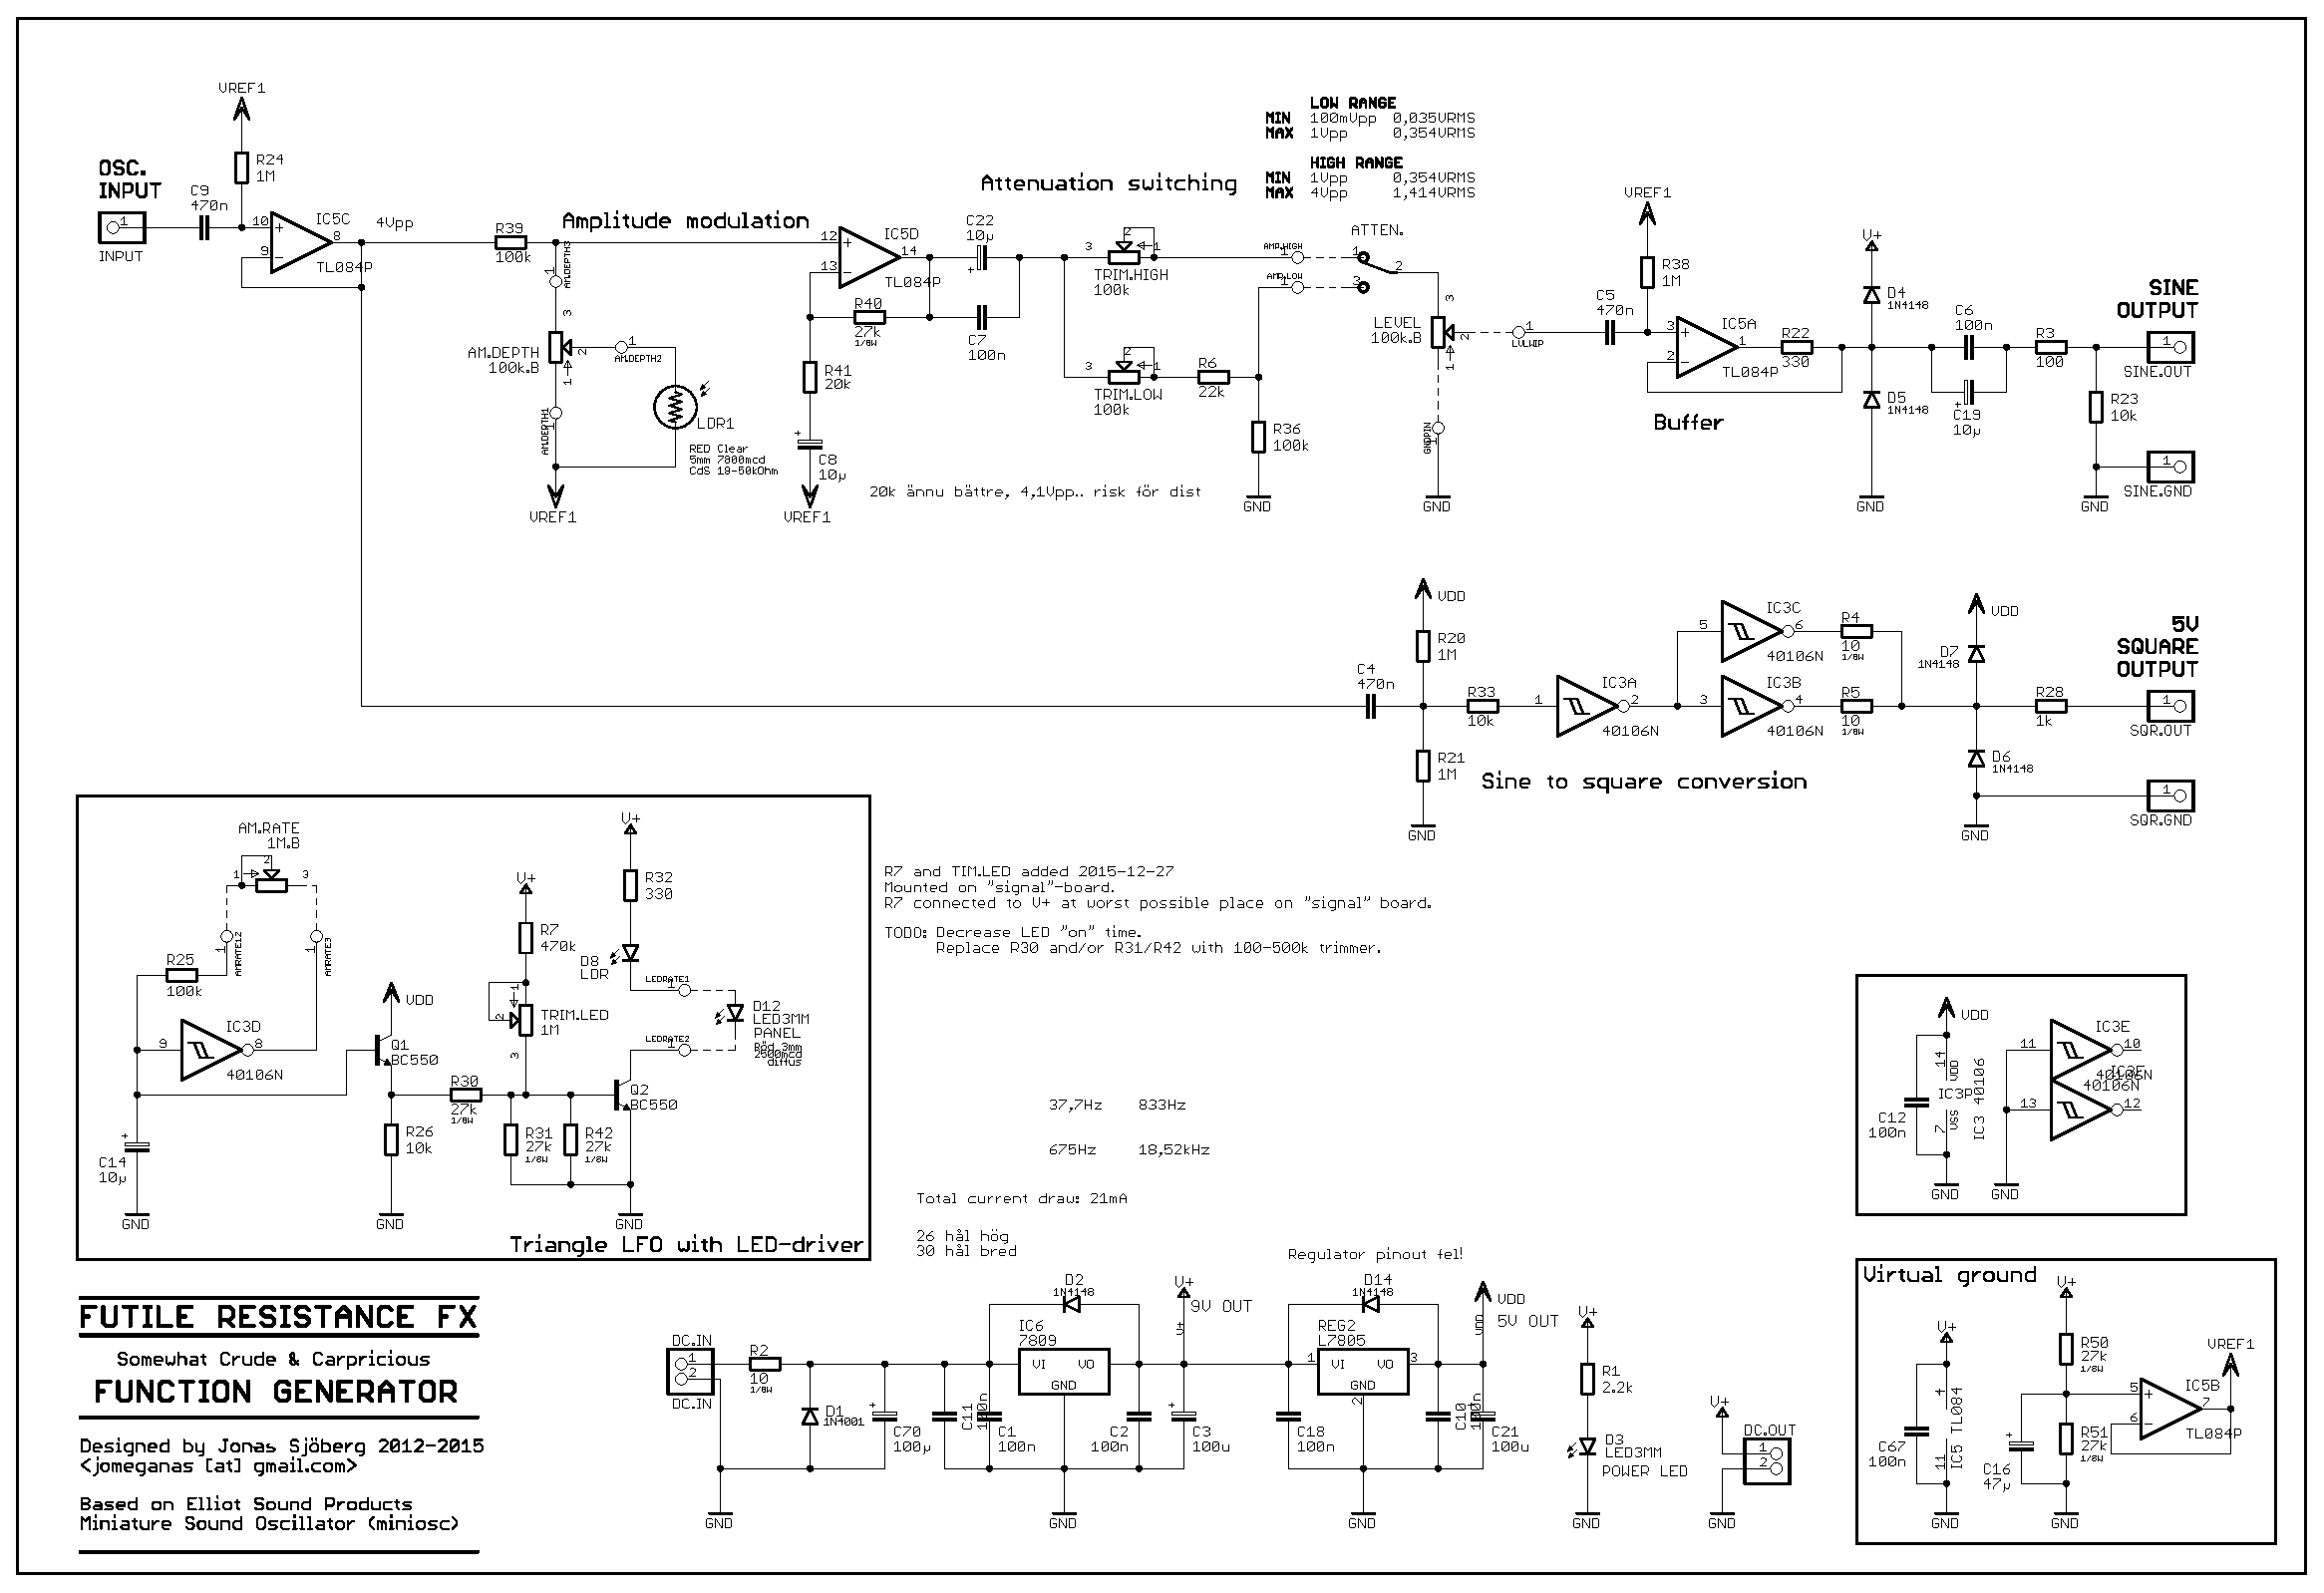
\includegraphics[width=\linewidth]{img/signal-generator_schematic-1}
  \caption{Kopplingsschema för signalgeneratorn som användes vid laborationen.}
  \label{fig:siggen-schem-1}
\end{sidewaysfigure}

\begin{sidewaysfigure}[ht]
  \centering
  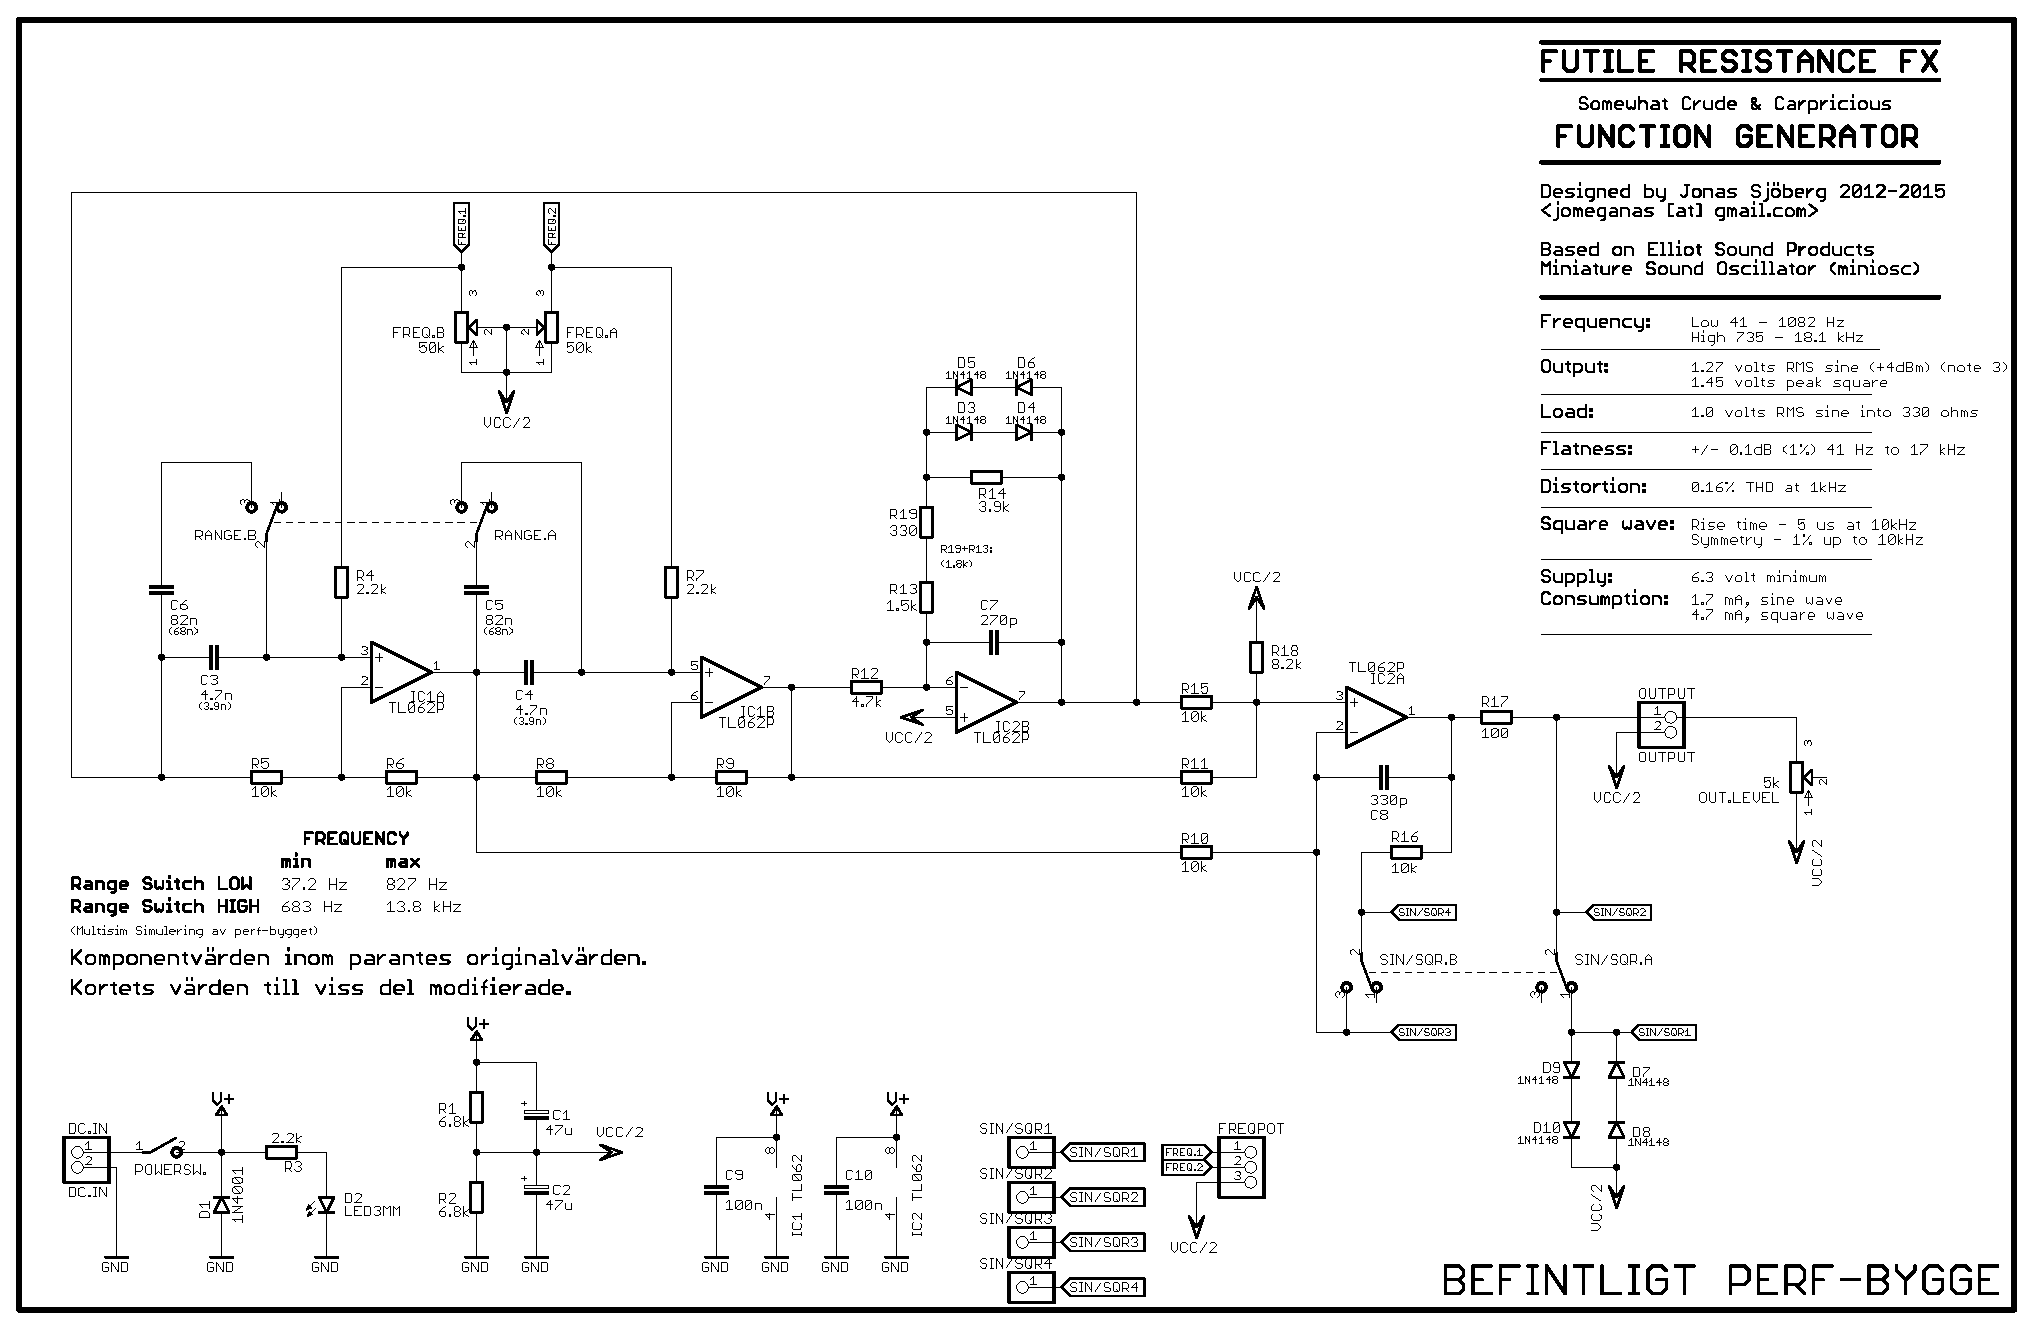
\includegraphics[width=\linewidth]{img/signal-generator_schematic-2}
  \caption{Kopplingsschema för signalgeneratorn som användes vid laborationen.
           Den här delen innehåller amplitudmodulering och trigger-utgången.}
  \label{fig:siggen-schem-2}
\end{sidewaysfigure}

